% Search for all the places that say "PUT SOMETHING HERE".

\documentclass[11pt]{article}
\usepackage{amsmath,textcomp,amssymb,geometry,graphicx,enumerate}
\usepackage{algorithm}
\usepackage{algorithmicx}
\usepackage{algpseudocode}
\usepackage{hyperref}
\usepackage{ctex}
\usepackage{listings}
\usepackage{xcolor}

\definecolor{codegreen}{rgb}{0,0.6,0}
\definecolor{codegray}{rgb}{0.5,0.5,0.5}
\definecolor{codepurple}{rgb}{0.58,0,0.82}
\definecolor{backcolour}{rgb}{0.95,0.95,0.92}
\lstdefinestyle{mystyle}{
	backgroundcolor=\color{backcolour},
	commentstyle=\color{codegreen},
	keywordstyle=\color{magenta},
	numberstyle=\tiny\color{codegray},
	stringstyle=\color{codepurple},
	basicstyle=\ttfamily\footnotesize,
	breakatwhitespace=false,
	breaklines=true,
	captionpos=b,
	keepspaces=true,
	numbers=left,
	numbersep=5pt,
	showspaces=false,
	showstringspaces=false,
	showtabs=false,
	tabsize=2
}

\lstset{style=mystyle}

\def\Name{周盈坤}  % Your name
\def\SID{201918013229046}  % Your student ID number
\def\Class{}
\def\le{\leqslant}
\def\logN{\log{}n}
\newcommand{\ro}[1]{\romannumeral #1}
\def\Session{20春季}
\renewcommand{\algorithmicrequire}{\textbf{input:}}
\renewcommand{\algorithmicensure}{\textbf{output:}}
\newcommand{\norm}[1]{\lVert #1 \rVert}
\title{大数据系统与大规模数据分析19-20春季大作业Proposal}
\author{汪钇丞\ 201928015029027\ \ 刘力玮 201928015059037 \\
		汪润川\ 201928013229149\ \ 胡登杭 201928015029028 \\
	\Name\ \ \SID}
\markboth{题目8:Serverless Computing学习}{题目8:Serverless Computing学习}
\pagestyle{myheadings}
\date{}

\newenvironment{qparts}{\begin{enumerate}[{(}a{)}]}{\end{enumerate}}
\def\endproofmark{$\Box$}
\newenvironment{proof}{\par{\bf Proof}:}{\endproofmark\smallskip}
\newcommand{\angleb}[1]{\langle #1 \rangle}

\textheight=9in
\textwidth=6.5in
\topmargin=-.75in
\oddsidemargin=0.25in
\evensidemargin=0.25in

\begin{document}
\maketitle

\section{Microsoft Serverless Computing}
\subsection{Azure (汪钇丞)}
Azure是微软的云平台,如图\ref{figs:Overview}所示,它根据不同层次的用户需求,提供了丰富和灵活的端到端服务\cite{overview}。Azure认为无服务器计算最主要的特点也是优点在于:开发者无需管理基础结构,而更多地专注于业务逻辑,能够在更短时间内交付更多功能;云服务提供商根据运行代码的工作负荷,自动预配、缩放和管理运行环境。Azure提供了符合上述特性的三种级别的抽象:Platform-as-a-Service(PaaS)、Functions-as-a-Service(FaaS)、Kubernetes-as-a-Service(KaaS),被认为是Azure的无服务器计算的三个主要组成部分。
\begin{figure}[!htbp]
	\centering
	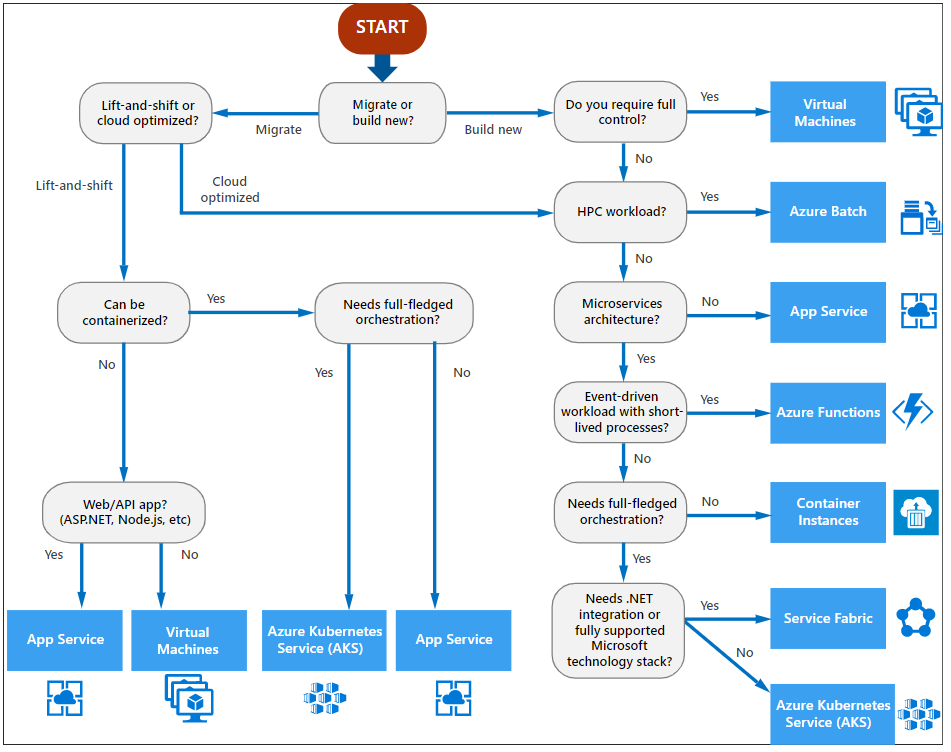
\includegraphics[scale=0.5]{figs/AzureChoice.PNG}
	\caption{Azure根据需求提供的功能选择(\cite{overview}图1)}
	\label{figs:Overview}
\end{figure}

\subsection{Azure App Service (汪钇丞)}
Azure App Service是Azure提供的平台即服务(PaaS),相比较与基础架构即服务(Infrastructure-as-a-Service)需要用户自行修补和备份服务器,安装软件包,更新操作系统和监视应用程序,Azure App Service中由运营商来做上述的工作来维护虚拟机环境,用户只需要选择一个基于HTTP请求的平台目标,例如Web应用,REST API,或者移动后端等。

随着应用对后台处理的需求增加,微软引入了Azure WebJobs作为Azure App Service的拓展。WebJobs 作为一个工作流程步骤,它含有基于时间的触发器,以及基于Azure提供的存储系统,数据库,消息队列等工具的触发器,可以持续执行,通过触发执行,或者是手动触发执行特定的逻辑任务。Azure WebJobs本身已经具有了一些典型无服务计算运行时的特点,可以说是一个FaaS平台的雏形,但WebJobs SDK的编写相对来说还是较为繁琐,监视和日志系统也不够完善。

相比较于其他PaaS平台,Azure App Service的特点在于可以支持包括ASP.NET,JAVA,Ruby,Node.js,PHP,Python在内的多种编程语言;能够使用微软自家Visual Studio中的专用工具,简化了创建,部署和调试工作;可以使用Azure的DevOps进行持续集成和部署;能够使用Azure Active Directory进行身份验证确保安全性;可以从Azure市场上获取到大量应用程序的模板。最关键的一点是,Azure App Service 除了在基本付费计划当中需要用户手动伸展和收缩集群,在标准和高级付费计划当中,都提供了自动化集群和实例数量伸缩的功能选项,让用户无需再关注应用运行环境,这一特点使得Azure App Service具有了无无服务器计算的性质。


\subsection{Azure Functions (汪钇丞)}
Azure Functions是Azure提供的函数级别的抽象(Function as a Service),一个典型的事件驱动型无服务计算运行时。如图\ref{figs:architecture}所示,Azure Functions建立在Azure App Service和WebJobs SDK的基础之上,相当于一个轻量级的WebJobs SDK脚本模型。它利用触发器自动执行代码以响应事件或绑定,能够根据工作负载量自动灵活地缩放计算资源,无需基础结构管理。相对于WebJobs只能跟随Azure App Service运行在公有云之上,Azure Functions既可以运行在Azure公有云上,也可以通过Azure Stack运行在自有混合云平台中,常常在Azure App Service 中作为服务的一部分。

\begin{figure}[!htbp]
	\centering
	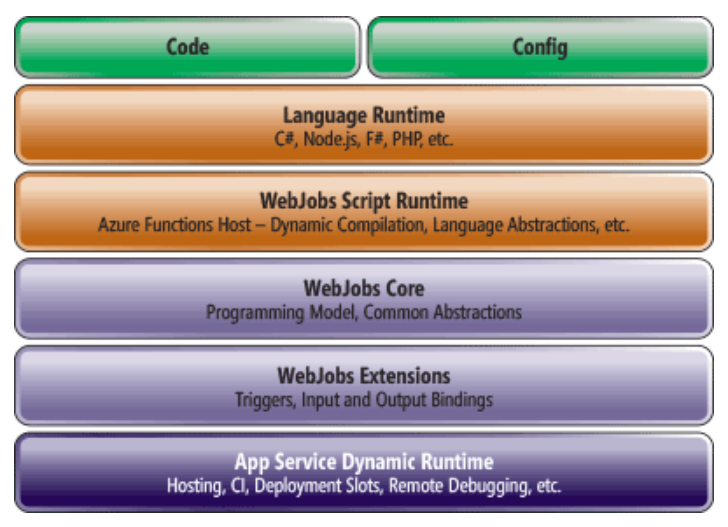
\includegraphics[scale=0.5]{figs/AzureArchitecture.PNG}
	\caption{Azure App Service体系结构(\cite{archi}图1)}
	\label{figs:architecture}
\end{figure}

\subsubsection{Azure Functions触发器(汪钇丞)}
触发器是启动函数的按钮,定义函数如何被调用,为请求提供标准的跨平台有效负载。每个函数有且只有一个触发器。Azure Functions可以响应的触发包括:
\begin{enumerate}
    \item HTTP:基于HTTP请求运行代码, Azure API Management将云服务的所有后端服务API网关中心化,可以集中接收HTTP请求。
    \item 计时器:基于时间调度在预定的时间执行代码,可以满足周期性的触发,用于监视系统等。
    \item 数据库:连接Azure的全球分布式的多模型NoSql数据库Azure Cosmos DB。基于该数据库文档的增删改情况运行代码。
    \item 存储系统:连接了Azure存储HTML,CSS等静态Web内容的Azure Blob存储,消息队列Azure Queue,表格Azure Table等。基于这些存储的增删改情况运行代码
    \item Event Grid:事件网格是Azure完全托管的事件路由服务,使用发布/订阅模型,收集和传递多个主题源发布的事件。基于事件网格订阅的一系列事件来进行反馈
    \item Event Hub:Azure面向loT领域收集设备和传感器数据的中心,基于物联网设备的大量数据输入,运行代码进行反馈
    \item 服务总线:连接其他Azure或者自有的服务以及设备,对总线中的消息队列等作出反馈
\end{enumerate}
\subsubsection{Azure Functions绑定(汪钇丞)}
Azure通过Azure Logic Apps以低编码/无编码的方式,集成连接了各类软件,应用以及Software as a Service等服务,使得Azure Functions可以直观的创建无服务器工作流,将云中的数据连接并集成,提供给Azure Functions当中作为工作负载。如图\ref{figs:bind}所示,Azure Functions通过显式声明的方式进行绑定,将另一个微软的资源连接到函数当中。绑定可以是输入绑定、输出绑定或者都绑定。绑定对于Azure Function是可选的,一个函数可能有一个或多个输入和输出绑定。绑定的输入可以来自Azure的存储系统,数据库,微软的表格,云盘等等。输出除前述的资源之外还可以是通向事件网格,物联网中心,微软的邮件系统等。
\begin{figure}[!htbp]
	\centering
	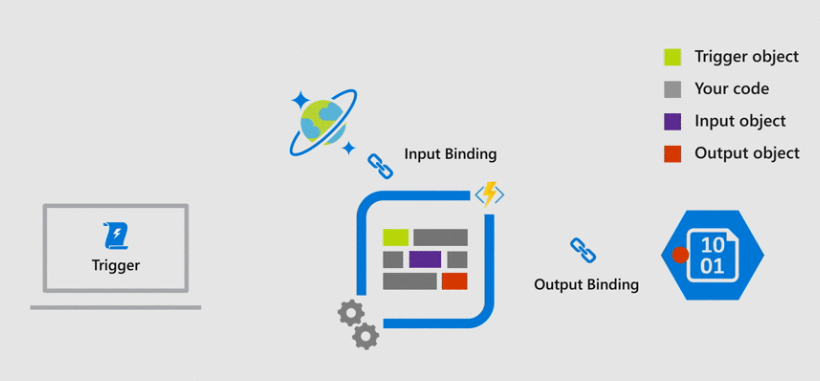
\includegraphics[scale=0.5]{figs/AzureBindings.png}
	\caption{Azure App Service体系结构(\cite{binding}图2)}
	\label{figs:bind}
\end{figure}
\subsubsection{Azure Functions安全和监控(汪钇丞)}
Azure Application Insights是一个无服务器诊断平台,作为Azure Monitor功能的一部分,内置在Azure Functions当中作为一种服务提供。它不需要额外配置服务器或设置库,自动与应用集成,负责监控和分析代码性能,可以收集日志,性能数据和错误信息,自动检测性能异常,诊断问题并了解函数的使用情况,给出解决意见。通过应用程序图和分布式跟踪,在应用程序的所有组件中发现任务热点,任务瓶颈和故障,并通过非常人性化的UI展示。除了内置的遥控跟踪可供控制,也可以自定义统计信息,设置日志级别,生成定制的遥控跟踪项目。

而作为Azure App Service的一部分,Azure Functions也是通过Azure Active Directory,或者Microsoft帐户和外部提供商的内置身份验证授予应用程序访问权限,并通过Azure Key Vault全面控制访问策略和审核历史记录。除此之外的Azure Functions的高级付费计划中提供了独立隔离的虚拟网络Azure VNet,可以限制进入的流量。Azure Security Center则负责预防、检测和响应威胁,增强对Azure 资源安全的可视化和可控性。
\subsubsection{Azure Functions的付费计划(汪钇丞)}
针对不同的应用场景和需求,Azure Functions提供了三种不同的付费计划,不同的计划也决定了函数的伸缩方式,每个函数实例的可用资源,以及对Azure VNet的可支持性。
\begin{itemize}
\setlength{\itemsep}{0pt}
\setlength{\parsep}{0pt}
\setlength{\parskip}{0pt}
    \item Consumption计划:最典型的无服务器计算付费计划,仅当函数运行时,基于执行的实例数量、执行时间和执行所用内存大小为计算资源付费。Azure会根据传入事件的数量动态添加和删除Azure Functions主机的实例,自动扩展
    \item Premium计划:适用于函数一直连续执行的情况,计划会保持至少一个永久热的实例在运行,以避免冷启动,意味着费用计算会有最低成本。除此以外用户可以选择连接Azure VNet,选择实例所用的CPU核数量,并拥有无限执行时间(至少60分钟)而不会超时
    \item Dedicated计划:实际上就是分享Azure App Service的资源,如果Azure App Service的付费计划中的虚拟机没有被充分利用,则用来创建Azure Functions实例。这也意味着虚拟机会一直在线。
\end{itemize}
Consumption计划和Premium计划根据创建的函数实例数来伸缩所需的CPU和内存资源,伸缩的单位就是一个函数实例,Azure Functions使用一个伸缩控制器监测触发事件,并启发式地控制伸缩大小,伸缩范围从0个实例到200个实例,每个实例可以处理很多个请求。对HTTP触发器每秒最多增加一个实例,而对非HTTP触发器最快每30秒增加一个实例。而Dedicated 计划则默认的是手动伸缩,也可以在对应App Service 计划中选择自动伸缩。另外Azure Functions依赖Azure存储来管理触发器和记录函数执行等,所以用户必须要有一个支持Azure Blob, Queue, Files, and Table storage的Azure存储账户。

\subsubsection{Azure Functions的性能(汪钇丞)}
Azure Functions作为微软的商用无服务器计算运行时,它的具体实现集成了众多Azure服务,并是不开源的。因而现有的相关论文的研究方法包括有:利用Azure的基本服务和工具,以及其他的开源项目有,重新搭建出一个FaaS的原型\cite{mcgrath2017serverless};或是直接测试Azure Functions 的进行测试,尝试逆向构建并了解其性能特点\cite{wang2018peeking}。

\cite{wang2018peeking}{\textit{Wang等人发表在USENIX ATC’18的文章}}对Azure Functions的性能和可用性进行了更深入的评测。他们首先根据官方文档找到了一个环境变量,由它能够确定Azure用于执行函数的虚拟机ID,论文使用两个不同的账号,分别触发500次函数,然而发现有30\%的函数实例是与另一用户的函数实例共存在同一个虚拟机上的。由于同一虚拟机共享相同的资源,这种共存情况为数据安全带来了一定隐患,会导致应用程序容易受到各种各样的边通道攻击。

而在更大规模的50000次的函数调用测试当中,论文总共统计到4104个不同的虚拟机,三种不同的CPU,以及有单核,双核,四核三种配置。根据Azure官方付费计划中的叙述,一个计划内可以最多拓展到200 个实例,但实际在测试当中,不论作者如何调整,整体的实例数也没有超过10个,且都不在同一个虚拟机上,说明Azure不会在同一虚拟机上申请相同函数的实例,造成绝大多数的申请都是由个别实例完成的。

当\cite{wang2018peeking}采用同一账户调用100个不同的函数,使总的函数实例数达到1000个时,论文查看所有实例的虚拟机分布,发现只有最多8个实例能够独享一台虚拟机,绝大部分的实例都会和其他实例共享虚拟机,并且大部分共享的虚拟机都是在单核环境,而不是在其他双核和四核虚拟机上。这表明Azure提供了更多的低性能单核虚拟机,而有实例共享虚拟机的情况都发生在单核虚拟机上,会带来更大的竞争。论文随后采用两个账户,一个触发少量函数实例扮演“受害者”,一个同时产生大量函数实例作为“侵略者”,作者发现有部分“受害者”的实例会和“侵略者”的实例共享虚拟机的情况,由此产生性能损失。

冷启动指的是未经使用或长时间没有使用的应用程序,由于需要重新分配和加载而启动时间较长的现象。在冷启动现象的测试中,\cite{wang2018peeking}对1000种不同的函数,连续调用两次,分别作为冷启动和热启动的比较。结果显示,和同类型的AWS和Google产品相比较,尽管Azure每个函数实例分配了更多内存,但冷启动延迟的中位数要远远高出,并且相对来说延迟时间更不稳定,如图\ref{figs:cold} 所示。而作者统计了一个函数实例在运行结束后到被回收掉的时间,发现Azure的回收间隔时间则相对较短,这意味着Azure的资源利用效率更高,但新的相同函数请求找到一个热实例的可能性更小。不过在存活实例的最长生命时间实验中,Azure函数实例在保持存活的情况下,在虚拟机中的最长存在时间要明显高于另外两个产品。
\begin{figure}[!htbp]
	\centering
	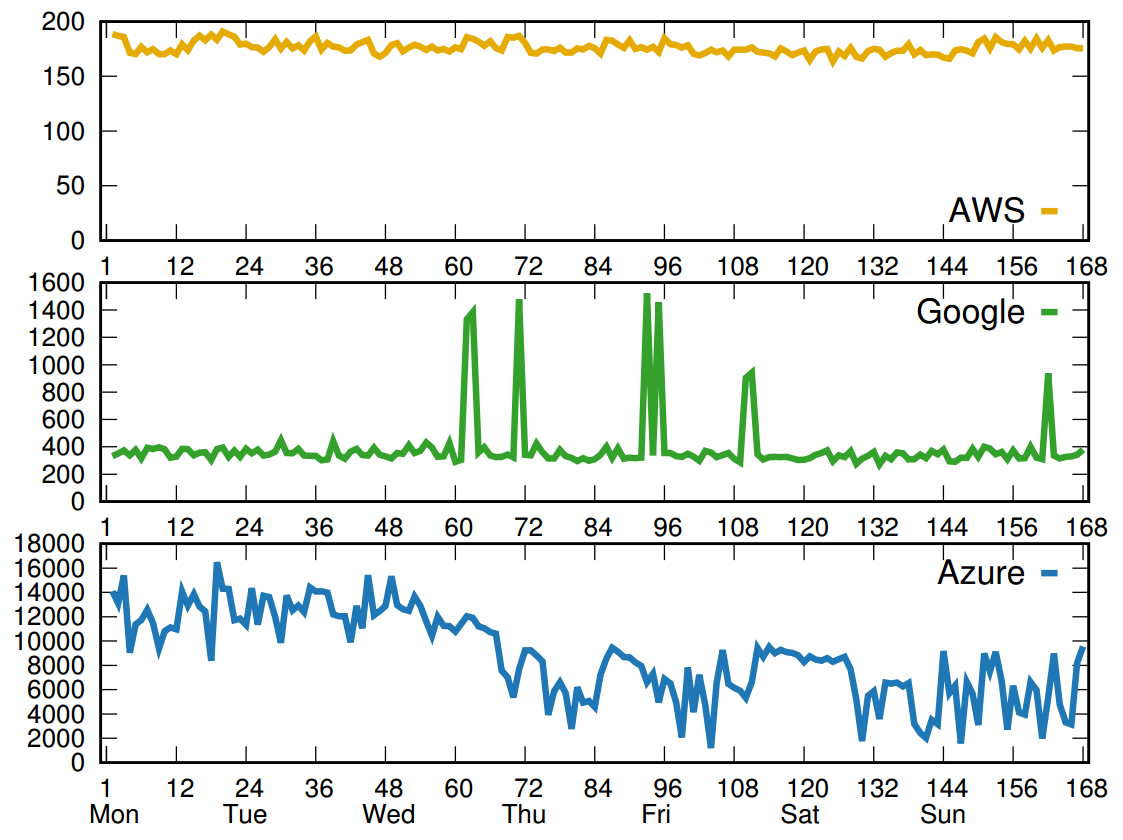
\includegraphics[scale=0.5]{figs/ColdStart.PNG}
	\caption{主流FaaS平台的冷启动延迟对比(\cite{wang2018peeking}图8)}
	\label{figs:cold}
\end{figure}
在单独的虚拟机性能方面,Azure的函数实例的CPU占用率,I/O,网络吞吐量方面和其他两款产品差异不大,但由于Azure提供的虚拟机并不一致,相对来说四核的虚拟机性能更佳,CPU资源占用率更高,而单个实例的I/O和网络吞吐会随着实例共享而下降。因而Azure Functions的性能相对来说并不稳定。

\cite{wang2018peeking}的测试都是针对Consumption计划,在论文撰写时Premium计划还没有推出。而Premium计划的提供已经解决了避免冷启动的问题,方法是至少保持一个热实例,也通过隔离的虚拟网络Azure VNet 和可配置的CPU核数量,保证了没有不同用户共享虚拟机的情况出现,避免了实例之间的竞争,虚拟机的性能也可以得到保证。论文在最后也说明最新的测试证明了Azure Functions更新的有效性。而Dedicated 计划则可以完全避免冷启动,因为虚拟机是由用户控制的,但这种情况之下就不再是无服务器的了。
\subsubsection{Durable Azure Functions(胡登杭)}

\subsection{Azure Kubernetes Service(汪钇丞)}
Kubernetes是一个用于自动部署,扩展和管理容器化应用程序的开源系统。它提供API来控制容器的运行方式和位置.自动进行服务发现、负载均衡、存储编排、部署和回滚、自我修复、跟踪资源分配和基于计算利用率进行扩展。而Azure Kubernetes Service(AKS)是Azure提供的Kubernetes即服务(KaaS),用于托管Kubernetes环境,使在Azure中部署和管理容器化的应用程序变得容易。由于不需要关注具体的容器管理,能够自主伸缩,因而AKS也被视为微软无服务器计算的一部分。
\subsubsection{Kubernetes结构(汪钇丞)}
Kubernetes的结构如图\ref{figs:Structure}所示,其结构的主要组成包括:
\begin{figure}[!htbp]
	\centering
	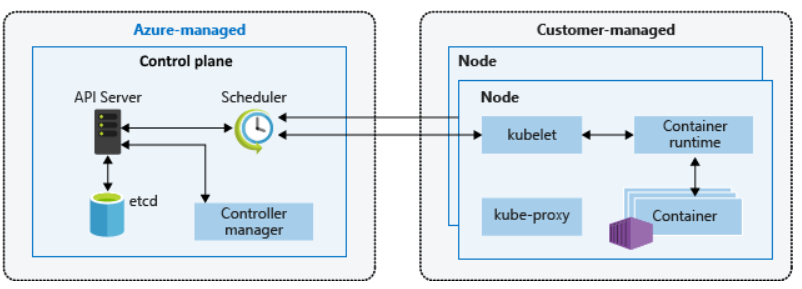
\includegraphics[scale=0.5]{figs/Kubernetes.PNG}
	\caption{Kubernetes的结构图(\cite{Kubernetes}图1)}
	\label{figs:Structure}
\end{figure}
\begin{itemize}
\setlength{\itemsep}{0pt}
\setlength{\parsep}{0pt}
\setlength{\parskip}{0pt}
    \item 控制平台:也就是主节点,由许多小型专门的控制循环和服务组成。其中API Server是底层Kubernetes API的公开方式。为管理工具(如kubectl或Kubernetes dashboard)提供交互;Cluster store是为维护Kubernetes集群状态和配置的一个高度可用的KV结构etcd存储;Scheduler在创建或扩展应用程序时,根据工作负载确定哪些节点可以运行并启动它们;Controller-Manager监督许多更小的控制器,提供自愈能力、扩容、应用生命周期管理、服务发现、路由、服务绑定和提供。
    \item Nodes节点:Kubernetes集群的工作节点,负责查看API服务器以获得新的工作分配,执行新的工作分配,并向控制平面报告。其中kubelet负责节点注册过程,监视API Server来得到分配的工作,并将容器的运行状态汇报给API Server;Container Runtime负责镜像管理以及Pod和容器的真正运行;kube-proxy负责为Service提供cluster内部的服务发现和负载均衡,通过iptables规则引导访问到服务IP,并将其重定向至正确的后端应用
    \item 容器都运行在Pod内部,而一个Pod运行一个应用的实例。Pod通常与容器进行1:1的映射,高级场景中一个Pod也可能包含多个容器。这些多容器容器被安排在同一个节点上,允许容器共享相关资源,相同的Pod将共享相同的IP 地址。创建一个Pod 时,可以定义资源请求来申请一定数量的CPU或内存资源。Scheduler尝试将pod调度到具有可用资源的节点上运行,以满足请求。Pod是伸缩的最小单元。如果要伸缩应用程序,可以添加或删除Pod,不能通过向现有的Pod添加更多容器。由于Pod是不可靠的,Pod的伸缩也可能很耗费IP地址,Service为Pods集合提供可靠的网络
\end{itemize}
\subsubsection{AKS特征(汪钇丞)}
AKS的控制平面由Azure来负责控制,并保证是单租户使用的,而只需为运行应用程序的Node付费,而集群的Node数量是至少3 个。受托管的控制平面意味着用户不需要配置高度可用的etcd存储等组件,但是它也意味着不能直接访问主节点。AKS建立在开源的Azure Kubernetes 服务引擎(AKS-Engine)之上,使用Moby作为容器运行时,在包含多个节点池的AKS集群中,需要告诉Kubernetes 调度器将哪个节点池用于给定的资源。相比于传统Kubernetes,AKS可以将Azure存储等工具连接到节点和Pods,可以使用GPU,可以利用之前提到的Azure Active Directory,监视和诊断之类的功能。另外AKS提供了虚拟节点,无需等待Kubernetes集群的自动缩放器部署VM计算节点,即可快速运行虚拟节点上热启动的Pod,而只为它们的执行时间付费。
\subsubsection{基于Kubernetes的事件驱动自动缩放(汪钇丞)}
基于Kubernetes的事件驱动自动缩放器(即KEDA),可以指定应用程序以事件驱动方式扩展,根据需要处理的事件数确定如何扩展Kubernetes中的任何容器。作为一个单一用途的轻量级组件,它可以添加到包括AKS在内的任何Kubernetes集群中,与标准Kubernetes组件一起使用,而不会覆盖或重复原有功能。KEDA自动伸缩,事件驱动的特点,与Azure Functions的性质吻合,因而安装KEDA的AKS也是Azure Functions的一种可用托管方式,通过Kubernetes中提供事件驱动的缩放。
\begin{figure}[!htbp]
	\centering
	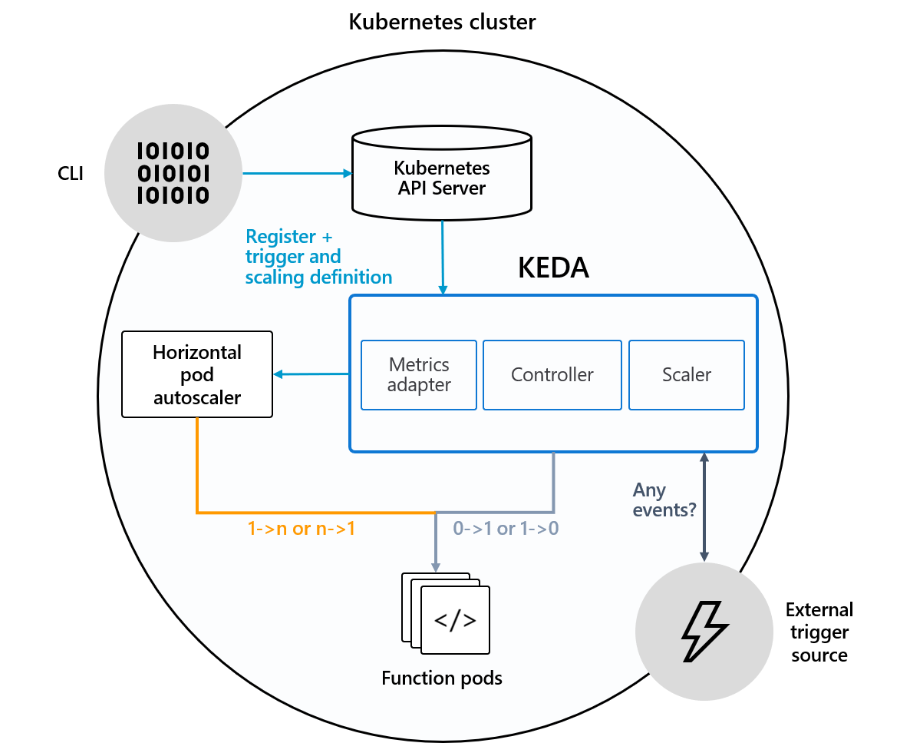
\includegraphics[scale=0.5]{figs/KEDA.PNG}
	\caption{Kubernetes的结构图(\cite{Kubernetes}图1)}
	\label{figs:KEDA}
\end{figure}
Kubernetes自身通过Horizo​​ntal Pod Autoscaler定期查询内存和CPU资源的利用率等评价指标来决定伸缩的程度,最终计算得到应该创建的实例数。而Kubernetes从1.6版本开始支持添加自定义的指标,KEDA将触发对象的状态,例如Azure消息队列的长度,定义为评价指标,添加到指标服务器中提供给Horizo​​ntal Pod Autoscaler,做到启发式的Pod实例伸缩。如图\ref{figs:KEDA} 所示,KEDA 的功能实现主要依靠三个组件:
\begin{enumerate}
    \item Scaler:通过自定义资源ScaledObject的manifest定义,和外部触发对象的工具连接,负责获取定义的指标并提供给指标服务器,KEDA支持同时插入多个Scaler
    \item Controller:负责初始部署,完成实例从0到1和从1到0,通过KEDA-operator容器驱动,在自定义的资源ScaledObject出现之后,创建一个Horizo​​ntal Pod Autoscaler。
    \item Metrics Adapter:即指标服务器,通过将Scaler提供的指标数据进行一定的处理,提供给相应的Horizo​​ntal Pod Autoscaler,由后者来根据指标对Pod实例数量进行伸缩。
\end{enumerate}
KEDA目前可支持的触发对象包括Azure存储队列,Azure服务总线队列,Azure时间网格,以及Apache Kafka等开源项目。但相比较于Azure Functions的原生计划来说还并不完整,如不支持计时器触发,HTTP请求等,或者是需要其他繁琐的插件来支持。
\bibliographystyle{alpha}
\bibliography{doc}
\end{document}

